\documentclass[a4paper, 11pt]{article}
	\usepackage[utf8]{inputenc}
    \usepackage[french]{babel}
    \usepackage[T1]{fontenc}
    \usepackage[top=3cm,, right=2cm,bottom=2cm,left=2cm]{geometry}
    \usepackage{eurosym} %pour le symbole euro

    \usepackage{tabularx}
    \usepackage{soul}
		\usepackage{enumitem}

		\usepackage{pdfpages}

    \title{Hackerspace Au Mans}
    \author{Procès-Verbal des Assemblées Générales Ordinaire et Extraordinaire}
    \date{Le jeudi 10 novembre 2016}

    \newcommand\sep{\noindent\rule{\linewidth}{.5pt}}

    \newcommand{\vote}[5]{

    \smallskip
    \fbox{\begin{minipage}[l]{\textwidth}
    	\smallskip
        \begin{center}
        	\ul{\textsc{Vote}}
        \end{center}

        #1\\
        \textbf{Votants} #2\\
        \textbf{Pour} #3\\
        \textbf{Contre} #4\\
        \textbf{NSPP} #5

        \smallskip

    \end{minipage}}
        \medskip
    }

    \newcommand\question[2]{\noindent\ul{\textit{\textsc{$\bullet$ #1}}}\\#2\\}

    %\ul{#2}}


\begin{document}

\maketitle

\section*{Préambule}

Le HAUM remercie \emph{la Ruche Numérique} pour le prêt de la salle pour cette réunion.

\section{Effectifs}

\begin{itemize}
	\item Présents :
		\begin{itemize}
      \item CONTY Romuald
      \item FAVREAU Tifenn
      \item BRETON Corentin
      \item PORTE Romain
      \item BEN ICHE Mehdi
      \item TOUCHARD Florent
      \item GABORIT Mathieu
      \item BRÉHÉRET Jérôme
      \item VANNIER Laurent
      \item VALLÉE Sébastien
      \item LEFRANÇOIS Jean-Marc
      \item MAURICE Fabien
      \item BIDAULT Bastien
      \item GABORIT-LEBREQUER Matthieu

		\end{itemize}
	\item Absents ayant donné procuration à CONTY Romuald :
		\begin{itemize}
			\item CHAINOT-BATAILLE Manuella
		\end{itemize}
	\item Absent ayant donné procuration à GABORIT Mathieu :
		\begin{itemize}
			\item BLAIN Fred
      \item DAZEL Olivier
		\end{itemize}
\item Absent ayant donné procuration à BRETON Corentin :
		\begin{itemize}
			\item BATAILLE Fabien
      \item GERVOT Suzy-Lou
		\end{itemize}
\item Absent ayant donné procuration à BRÉHÉRET Jérôme :
		\begin{itemize}
			\item DUTHÉ Yannick
		\end{itemize}
\item Absent ayant donné procuration à TOUCHARD Florent :
		\begin{itemize}
			\item COSTE Jérôme
			\item COFFIGNAL Alexandre
		\end{itemize}
\item Absent ayant donné procuration à PORTE Romain :
		\begin{itemize}
			\item ROUSSEAU Wojciech
		\end{itemize}
\end{itemize}

\bigskip

\section{Assemblée générale extraordinaire}
\textbf{La séance est ouverte à 19h30}

Cette assemblée générale extraordinaire a pour but d'ajouter la mention
\emph{prestations de services} à l'article 5 des statuts (Ressources) pour refleter
au mieux nos ressources.

\vote{Ajout de la mention manquante au statuts}{23}{23}{0}{0}

\textbf{La séance est levée à 19h32}

%%La présidence actuelle décide d'accorder le droit de vote à tous les présents pour la durée de cette AG.
\setlist{nosep,after=\vspace{\bigskipamount}}

\section{Assemblée générale ordinaire}
\textbf{La séance est ouverte à 19h32}
\subsection{Rapport Moral}

Le rapport moral (cf annexe) est présenté par le président.

\vote{Rapport moral}{23}{23}{0}{0}

Le rapport moral est validé par l'assemblée.

\subsubsection{Questions et remarques à propos du rapport moral}

Au niveau des partenariats, on peut ajouter à ceux présents dans le rapport moral,
sans être exhaustifs :
\begin{itemize}
	\item L'IMIE
	\item ST Microelectronics
	\item AgileMans
\end{itemize}

De même, concernant les évènements auxquels nous avons pu prendre part, on peut
ajouter :
\begin{itemize}
	\item La Global Game Jam
	\item AgileMans
	\item Bienvenus sur Mars
	\item La Gamers Assembly
\end{itemize}

Et pour les projets menés, des ateliers \og{Confection \& nouvelles
technologies}\fg{} ont été menés grâce à Tifenn et à AniBlue. Il a été décidé
de ne pas donner suite à ces ateliers.
\newpage{}
\question{Quelle sont nos obligations en vue du prochain local, ainsi que
pour le déménagement ?}{"Les conditions d'accès au nouveau local et à la suite
de la CICO sont les mêmes qu'aujourd'hui. Notre implication dans la CICO n'est
donc soumis à aucun engagement sinon celui moral de déménager à la proposition
d'un nouveau local. L'engagement du HAUM est donc la somme des engagements de ses
membres dans le projet."}

Il est à noter que \og{}La non fiabilité des informations entendues ne
permettait pas de transférer de vraies informations aux membres du HAUM lors
des discussions autour de ce projet.\fg{}

De même, \og{}Les informations "de couloir" ne sont pas relayées, seules les
informations récupérées dans un cadre officiel sont avérées.\fg{}

\question{Est il pertinent de lancer des sessions de formation ?}{Non, on va
préférer une approche moins typée FabLab et plus HackerSpace avec des \og{petites}\fg{}
formations pour mieux cibler les besoins et les personnes.}

\subsection{Rapport Financier}

Le trésorier présente le rapport financier (cf annexe).

\vote{Rapport Financier}{23}{23}{0}{0}

Le rapport financier est validé par l'assemblée.

\subsubsection{Question et remarques sur le rapport financier}

On note quelques prestations rétribuées (Gamers Assembly, Teriaki, Bienvenus
sur Mars), ce qui contribue à la très bonne santé des comptes cette année.
La vente de T-Shirt permet, elle aussi, de rapporter un peu d'argent.

Une enveloppe budgétaire est prévue pour avoir une connexion Internet au local,
ainsi que pour proposer une collation aux différents évènements proposés par le
HAUM.

%====================================================================================

\subsection{Cotisation}

Il est proposé de laisser la cotisation à 30\euro{} pour l'année 2017.

\vote{Cotisation à 30\euro{} pour l'année 2017}{23}{23}{0}{0}

La cotisation sera donc de 30\euro{} pour l'année 2017.

\subsection{Questions diverses}

\question{Serait il possible d'organiser des réunions de bureau régulières
(mensuelles, idéalement), avec les actifs de l'association ?}{Oui, la date de
la première réunion est fixée au deuxième mercredi de chaque mois, à 21H.}
\question{Doit on continuer l'écriture des résumés de séance ?}{Cette façon de
procéder ne fonctionne pas. Les réunions mensuelles évoquées précédement
devraient combler ce besoin. Il est aussi proposer de mettre en place un
\og{index des projets}\fg{} pour avoir une meilleure visibilité sur l'avancée des
projets en cours.}
\question{Doit on garder la do-ocracy ?}{Oui, évidement, mais sans aller jusqu'à
l'extrémisme (Article 11 des statuts de l'association : L'association fonctionne
par consensus.)}

\subsection{Election du bureau}

Se présentent à l'élection au bureau :

\begin{itemize}
  \item GABORIT-LEBREQUER Matthieu
	\item GABORIT Mathieu
	\item BRETON Corentin
	\item BREHERET Jérôme
	\item LEFRANCOIS Jean-Marc
	\item CONTY Romuald
	\item PORTE Romain
	\item BEN-ICHE Mehdi
	\item VANNIER Laurent
	\item FAVREAU Tifenn
	\item BLAIN Fred
	\item VALLÉE Sébastien
\end{itemize}

\\
   \hspace{-1cm} \fbox{\begin{minipage}{1.06\textwidth}
    		\smallskip
       		\begin{center}
        		\ul{\textsc{Vote}}\\
        		Élection au bureau de
      	 	\end{center}

       		\begin{tabularx}{2\textwidth}{p{2.6cm} | p{2.6cm} | p{2.6cm} | p{2.6cm} | p{2.6cm} | p{2.6cm} }
						\small \textsc{\mbox{GABORIT}-\mbox{LEBREQUER}} Matthieu &
						\small \textsc{GABORIT} \mbox{Mathieu} &
						\small \textsc{BRETON} \mbox{Corentin} &
						\small \textsc{BRÉHÉRET} \mbox{Jérôme} &
						\small \textsc{LEFRANÇOIS} \mbox{Jean-Marc} &
						\small \textsc{CONTY} \mbox{Romuald}
						\\
						\small \textbf{Votants} 24 &
						\small \textbf{Votants} 24 &
						\small \textbf{Votants} 24 &
						\small \textbf{Votants} 24 &
						\small \textbf{Votants} 24 &
						\small \textbf{Votants} 24
						\\
       		 	\textbf{Pour} 24 &
						\textbf{Pour} 24 &
						\textbf{Pour} 24 &
						\textbf{Pour} 24 &
						\textbf{Pour} 24 &
						\textbf{Pour} 24
						\\
        		\textbf{Contre} 0 &
						\textbf{Contre} 0 &
						\textbf{Contre} 0 &
						\textbf{Contre} 0 &
						\textbf{Contre} 0 &
						\textbf{Contre} 0
						\\
						\textbf{NSPP} 0 &
						\textbf{NSPP} 0 &
						\textbf{NSPP} 0 &
						\textbf{NSPP} 0 &
						\textbf{NSPP} 0 &
						\textbf{NSPP} 0
						\\
            \smallskip
    		\end{tabularx}




    \end{minipage}

    }
        \medskip

				\\
				\hspace{-1cm} \fbox{\begin{minipage}{1.06\textwidth}
		     		\smallskip
		        		\begin{center}
		         		\ul{\textsc{Vote}}\\
		         		Élection au bureau de
		       	 	\end{center}

		        		\begin{tabularx}{2\textwidth}{p{2.6cm} | p{2.6cm} | p{2.6cm} | p{2.6cm} | p{2.6cm} | p{2.6cm} }
		 						\small \textsc{PORTE} \mbox{Romain} &
		 						\small \textsc{BEN-ICHE} \mbox{Mehdi} &
		 						\small \textsc{VANNIER} \mbox{Laurent} &
		 						\small \textsc{FAVREAU} \mbox{Tifenn} &
		 						\small \textsc{BLAIN} \mbox{Fred} &
		 						\small \textsc{VALLÉE} \mbox{Sébastien}
		 						\\
		 						\small \textbf{Votants} 24 &
		 						\small \textbf{Votants} 24 &
		 						\small \textbf{Votants} 24 &
		 						\small \textbf{Votants} 24 &
		 						\small \textbf{Votants} 24 &
		 						\small \textbf{Votants} 24
		 						\\
		        		\textbf{Pour} 24 &
		 						\textbf{Pour} 24 &
		 						\textbf{Pour} 24 &
		 						\textbf{Pour} 24 &
		 						\textbf{Pour} 24 &
		 						\textbf{Pour} 24
		 						\\
		         		\textbf{Contre} 0 &
		 						\textbf{Contre} 0 &
		 						\textbf{Contre} 0 &
		 						\textbf{Contre} 0 &
		 						\textbf{Contre} 0 &
		 						\textbf{Contre} 0
		 						\\
		 						\textbf{NSPP} 0 &
		 						\textbf{NSPP} 0 &
		 						\textbf{NSPP} 0 &
		 						\textbf{NSPP} 0 &
		 						\textbf{NSPP} 0 &
		 						\textbf{NSPP} 0
		 						\\
		             \smallskip
		     		\end{tabularx}




		     \end{minipage}

		     }
		         \medskip

\textbf{La séance est levée à 21h46}

\section{Réunion de bureau}

Alors que l'ensemble des membres du nouveau bureau sont présents, il est décidé de procéder dans l'immédiat aux élections internes à celui-ci. Pour les votes suivants, le collège électoral est réduit au bureau seul (soient 9 membres).

\vote{Romuald CONTY au poste de président}{12}{12}{0}{0}
\vote{Mathieu GABORIT au poste de vice-président}{12}{12}{0}{0}
\vote{Jérôme BRÉHERET au poste de vice-président}{12}{12}{0}{0}
\vote{Sébastien VALLÉE au poste de vice-président}{12}{12}{0}{0}
\vote{Fred BLAIN au poste de vice-président et chargé de communication}{12}{12}{0}{0}

\vote{Tifenn FAVREAU au poste de trésorière}{12}{12}{0}{0}
\vote{Matthieu GABORIT au poste de vice-trésorier}{12}{12}{0}{0}

\vote{Jean-Marc LEFRANÇOIS au poste de secrétaire}{12}{12}{0}{0}
\vote{Laurent VANNIER au poste de vice-secrétaire}{12}{12}{0}{0}

\vote{Romain PORTE au poste de chargé de communication}{12}{12}{0}{0}
\vote{Mehdi BEN-ICHE au poste de chargé de communication}{12}{12}{0}{0}

\vote{Corentin BRETON au poste de chargé de gestion de projet}{12}{12}{0}{0}

\section{Composition du bureau}
\begin{description}
  \item[Président] Romuald CONTY
  \item[Vice-Président] \hfill
  	\begin{itemize}
        \item Mathieu GABORIT
  			\item Jérôme BRÉHERET
				\item Sébastien VALLÉE
				\item Fred BLAIN
			\end{itemize}
  \item[Trésorière] Tifenn FAVREAU
  \item[Vice-Trésorier] Matthieu GABORIT
  \item[Secrétaire] Jean-Marc LEFRANÇOIS
	\item[Vice-Secrétaire] Laurent VANNIER
  \item[Membres du bureau] \hfill
  	\begin{itemize}
        \item Corentin BRETON
        \item Romain PORTE
				\item Mehdi BEN-ICHE
    \end{itemize}
\end{description}
\bigskip
\textbf{La séance est levée à 22h.}

\bigskip\bigskip

\sep

\bigskip\bigskip

Le présent procès-verbal est approuvé par le président du HAUM.

\bigskip\bigskip

Président :



\newpage

\section{Rapport Moral}

\subsection{Bilan}

Cette année a été riche en changements et en actions menées pour et par l'association.

\subsubsection{Changement de local}

Après près de 2 ans dans nos anciens locaux au sein de la pépinière de la Ruche Numérique, le HAUM commençait à se sentir à l'étroit. Pour que les séances se déroulent dans les meilleures conditions de confort et de sécurité, il était temps de changer de local.

Cette envie a pu se concrétiser grâce au concours de Le Mans Développement, agence de développement économique de la métropole, qui a mis a notre disposition un local 2 fois et demi plus grand (passant donc de 29m\textsuperscript{2} à plus de 70m\textsuperscript{2}). Le Mans Développement a également réalisé les travaux nécessaires à l'installation de l'association et nous a mis en relation avec les services techniques de la ville du Mans pour que nous puissions récupérer du mobilier mis au rebut et ainsi meubler le lieu.

L'établi du HAUM est toujours mis à sa disposition par la Ruche Numérique malgré notre départ de leurs locaux.

Le bureau tient à remercier tous les acteurs institutionnels et les bénévoles qui ont rendu possible ce déménagement.

\subsubsection{Évolution des adhésions}

Au cours de l'année 2016, le nombre d'adhésions est passé de 35 à 41.
Il est à noter qu'environ 25 membres de l'année précédente n'ont pas renouvelé leur adhésion. L'association a par conséquent connu un changement massif de sa base de membres.

\subsubsection{Participation au projet French Tech}

Les discussions pour le changement de local font partie d'un projet plus vaste de création d'un pôle d'activité sur le secteur de la Gare dans le cadre du label French Tech. L'objectif est de mettre en oeuvre une Cité de l'Innovation Colaborative (CICO) rassemblant un certain nombre d'acteurs. L'inclusion du HAUM dans le projet (en tout cas sa présence sur le lieu de l'éventuelle CICO) a permis au Mans d'obtenir le label French Tech.

Dans le cadre de ce projet, les discussions portent à la fois sur la réhabilitation de l'ancien hôpital spécialisé de la rue Étoc Demazy mais également sur une "première phase" à plus court terme qui prendrait place dans les locaux de l'ancienne DDCS (Boulevard Lefaucheux). Cet aménagement permettrait de rassembler un incubateur, une pépinière et le hackerspace dans 1000m\textsuperscript{2}.

L'implication principale porte sur le déménagement du HAUM à court ou moyen terme. Il va donc être nécessaire de planifier ce déménagement, afin de minimiser les éventuels problèmes lors de celui-ci.

Cette planification ne peut se faire qu'avec le concours des partenaires institutionnels qui tendent à partager difficilement les informations. Affaire à suivre.

\subsubsection{Animations publiques}

Comme à l'accoutumée, le HAUM a contribué \& organisé en 2016, plusieurs animations à destination du public.

\paragraph{24H du code} Pour l'édition 2016 des 24H du Code (co-organisées par l'ENSIM et la Ruche Numérique), le HAUM a proposé un sujet. Le sujet portait sur la création d'un outil pour explorer des données fournies par Sarthe Développement (ouverture des lieux touristiques). Plusieurs membres du HAUM ont ainsi collaborer pour rédiger le sujet mais aussi être présent toute la nuit aux 24h du code pour guider les équipes.

\paragraph{Bienvenus sur Mars} Organisé au prieuré de Vivoin, le festival BienVenus sur Mars a invité le HAUM a présenter son Pong1D, le dHAUM mais également une création originale. Les Laumios sont nés ainsi et ont engendré de nombreuses idées de projets futurs. La vente de Laumios n'est pas exclue et l'affaire est à suivre.

\paragraph{Gamers Assembly} La Gamers Assembly accueille depuis 2 ans un village \textit{maker}. Cette année, l'organisation a convié le HAUM pour y présenter quelques réalisations. Ce fut l'occasion pour certains de nos membres d'aller pour la première fois sur une aussi grosse manifestation.

\paragraph{Siestes Teriaki} Après les siestes il y a deux ans et le festival l'an dernier, le HAUM est revenu à Teriaki cette année avec le projet Lampes Orbitales (également présenté à Vivoin), un mini-spectacles sur Laumios et un labyrinthe géant. L'organisation de l'évènement a posé de nombreux problèmes de gestion du temps et la question se pose désormais : doit on continuer à prendre part à des manifestations demandant autant de travail ?

\paragraph{Le sHAUM} Suite à son déménagement, le hackerspace a invité ses partenaires à venir découvrir le nouveau lieu. Ce fut une bonne occasion pour discuter avec toutes et tous et de faire découvrir l'association et ses possibilités.

\paragraph{Les HAUMTalks} L'association a organisé 6 sessions de ses mini-conférences en 2016 et au moins une septième est prévue. Les HAUMTalks intéressent un public assez large et permettent à chacun de présenter des sujets lui tenant à coeur (hacker). Ces rencontres permettent aussi de faire connaître l'association auprès d'extérieurs.

\subsubsection{Partenariats et Réseau}

Dans le cadre des différentes manifestations auxquelles il a participé et des différents projets auxquels il prend part, le HAUM continue de développer un réseau d'acteurs et de partenaires proches. Parmi eux : Teriaki, le Hangar Créalab, la compagnie Organic Orchestra, le CESI, la Ruche Numérique, l'ENSIM, la CCI du Mans et de la Sarthe, Le Mans Développement, Sarthe Développement, Le Mans Métropole, etc...

Merci à eux.

Le HAUM a pu participer à la Gamers Assembly 2016 grâce à l'association Rurart. L'association tient également à remercier QuaiLab, Les Usines Nouvelles et les petits débrouillards Poitou-Charente pour leur accueil et les échanges durant l'évènement.

\subsubsection{Projets}

Parmi les très nombreux travaux menés en séance, nous retiendrons tout particulièrement :

\begin{itemize}
    \item Lampes orbitales/Laumios
    \item LaumioAnimator
    \item Labyrinthe Initiati
    \item Améliorations de la fraiseuse
    \item Stations de soudage
    \item sHAUM
    \item Amélioration du 1DPong (lors de la Gamer's Assembly)
    \item Reconstruction du PianoStairs
\end{itemize}

Ces différents projet permettent de faire vivre et connaître l'association. Merci à tous ceux qui y ont pris part en les construisant, en les documentant, en les \textit{hackant} et en les faisant évoluer.

\subsubsection{Communication}

Depuis sa création officielle en 2012, le HAUM souffre de problèmes chroniques de communication. En effet, qu'elle soit à destination des membres ou des extérieurs, la communication du HAUM reste spécifique et non-inclusive.

À toutes fins utiles, le bureau tient à rappeler que le moyen de communication officiel de l'association est la liste de discussion par mail.

Les problèmes de communication ont notamment conduits à des malentendus avec nos partenaires, des retards dans la propagation de l'information et des soucis d'organisation plus larges. À l'échelle du hackerspace, la communication trop sporadique entre les membres a privé certains d'opportunités intéressantes et mené d'autres à s'écarter de l'association ou en tout cas des rôles qu'ils y occupaient.

À un autre égard, le manque de réponse sur l'adresse contact cause de graves lenteurs dans nos rapports aux autres et renvoie une image très statique du HAUM.

À l'avenir, il pourrait être intéressant de désigner 2 personnes responsables de \texttt{contact@haum.org} (tout en étendant la diffusion pour information au bureau) de même qu'il est nécessaire d'améliorer rapidement la communication des informations au sein de l'association. Les personnes en charge des relations avec les partenaires extérieurs \textbf{doivent} s'acquitter du transfert de l'information vers la mailing-liste (et pas uniquement en séance). Les informations importante, même confidentielles, doivent également être transférées \textit{a minima} sur la liste du bureau, sinon évoquées en réunion de bureau.

La vie du hackerspace est une affaire commune, ses relations vers l'extérieur également.

\subsection{Objectifs}

L'année 2016 a vu naître et progresser bon nombre de partenariats et de discussion. Il est donc raisonnable d'espérer que 2017 apportera son lot de nouveau matériel et de nouvelles relations.

Il est temps également de travailler sur l'axe de mutualisation des moyens pour que chacun des membres puisse réaliser ses envies et qu'un minimum d'argent soit perdu en doublons.

Le déménagement a entrainé la perte de l'accès à Internet et il est également nécessaire de remédier à cela dans les mois à venir pour garantir à tous un accès convenable aux ressources.

Les prestations et actions extérieures sont bien sûr à poursuivre et à encourager. Il faudra par ailleurs simplifier les relations avec les partenaires afin d'éviter les malentendus encore trop courants. La réalisation de prestations contribue au financement de l'association et il est souhaitable qu'un maximum de membres y participent.

Enfin, parce que l'association compte toujours plus de membres, il faudra travailler à l'amélioration des locaux pour permettre de l'utiliser comme lieu de travail bien sûr mais également comme lieu de vie et d'échange. Le HAUM vise à proposer une vision alternative du rapport à la technologie et si cela passe bien sûr par les aspects techniques, cela peut également être renforcé par des temps d'échanges informels (Jeudi du Libre) ou non (HAUMTalks).

\newpage

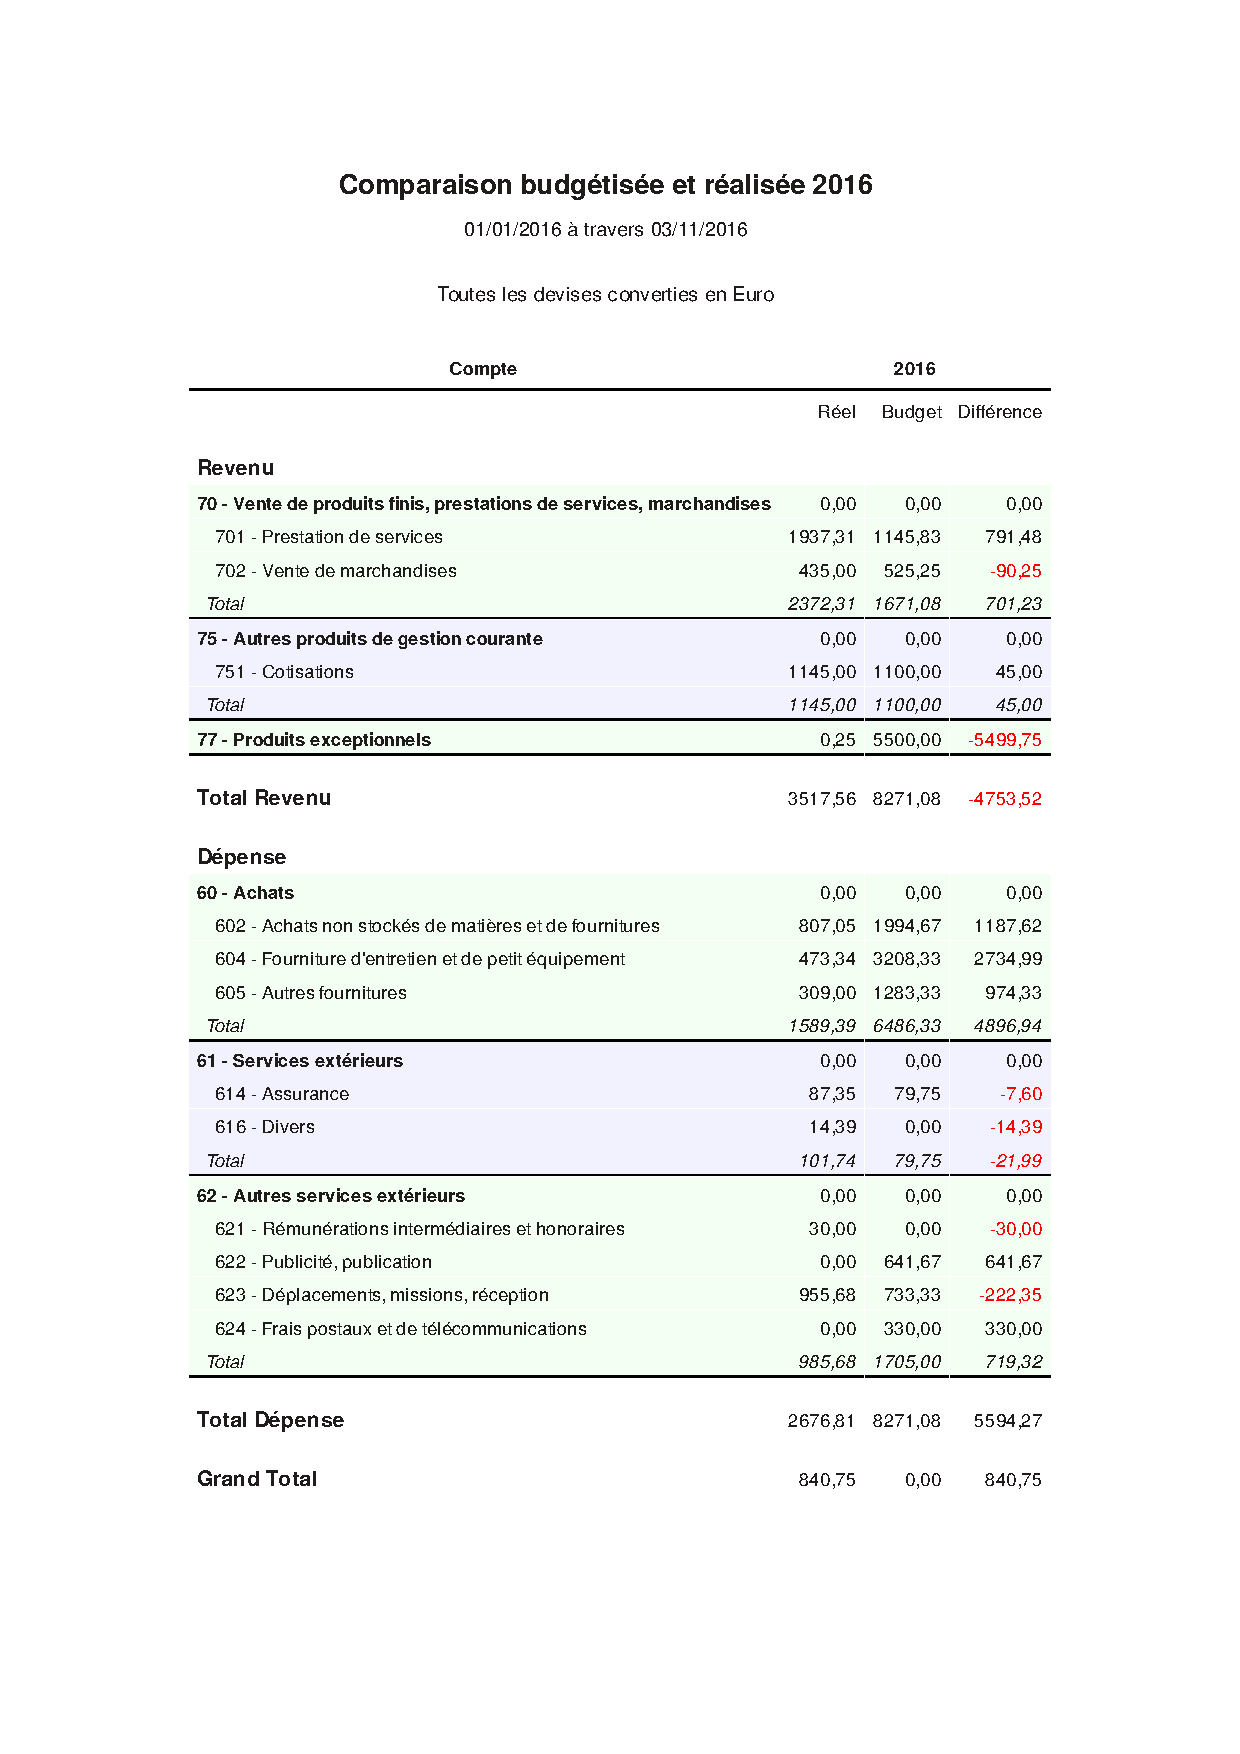
\includepdf[pages=-]{../convocation/BilanFinancier2016.pdf}
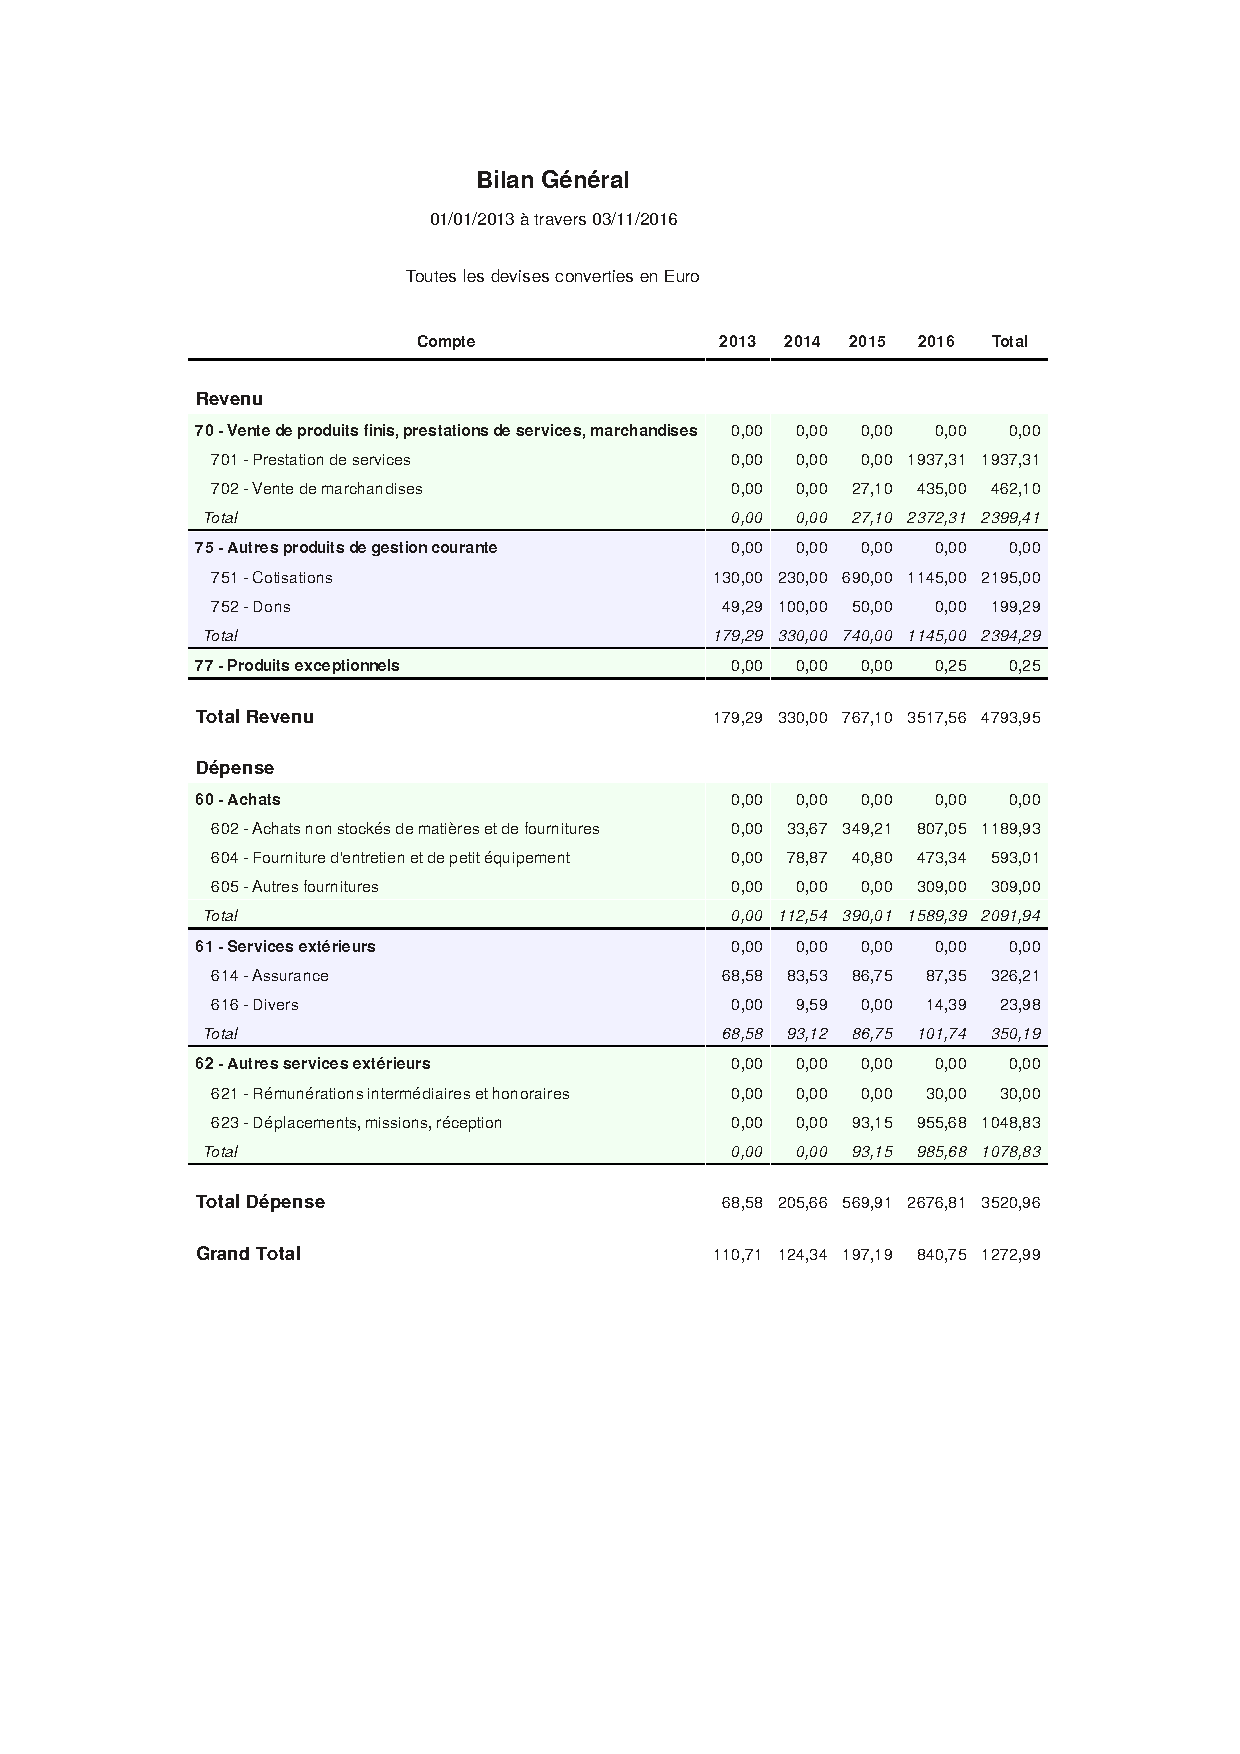
\includepdf[pages=-]{../convocation/BilanGeneral2016.pdf}
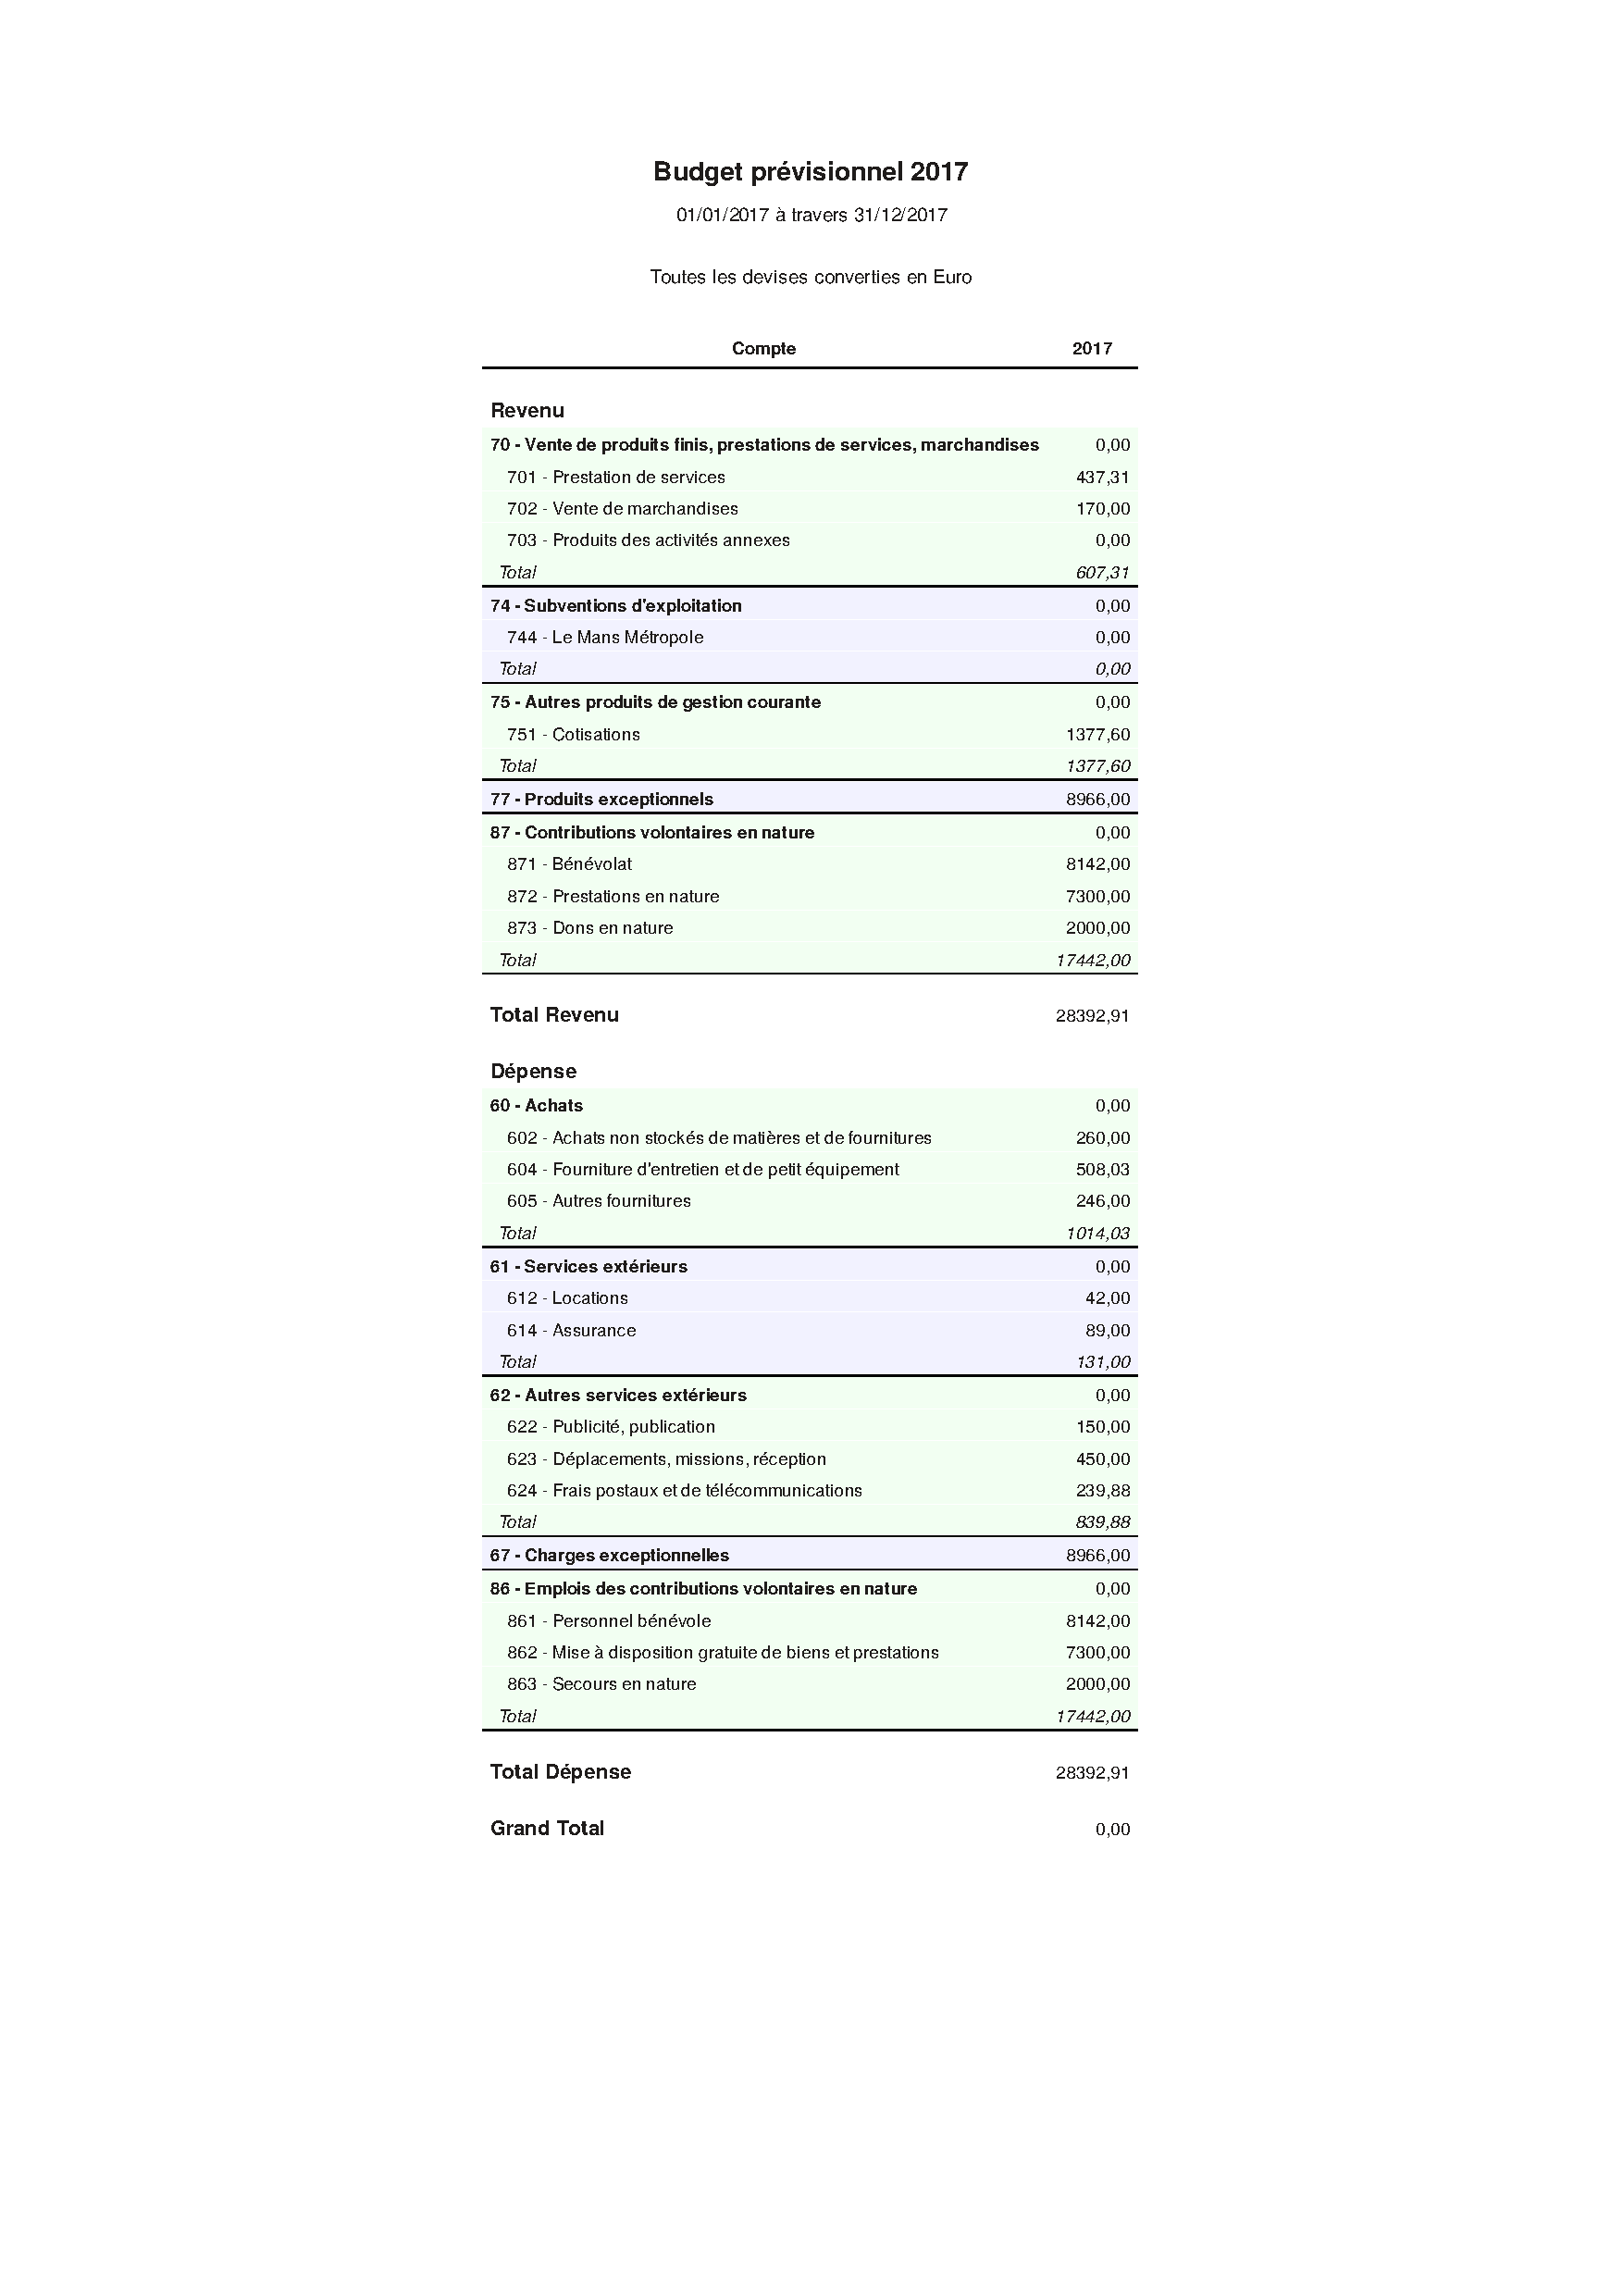
\includepdf[pages=-]{../convocation/BudgetPrevisionnel2017.pdf}
